\section{Protótipo}

Com base nos dados levantados, no processo definido e levando em consideração
as recomendações da IN4, foi projetado um documento que controla os principais
aspectos da gerência de uma ordem de serviço.

A primeira parte desse documento, representada pela Figura \ref{fig:cabecalho_1_2}
mostra a disposição do cabeçalho do mesmo e algumas informações básicas de 
identificação de uma ordem de serviço.

\begin{figure}[H]
  \centering
  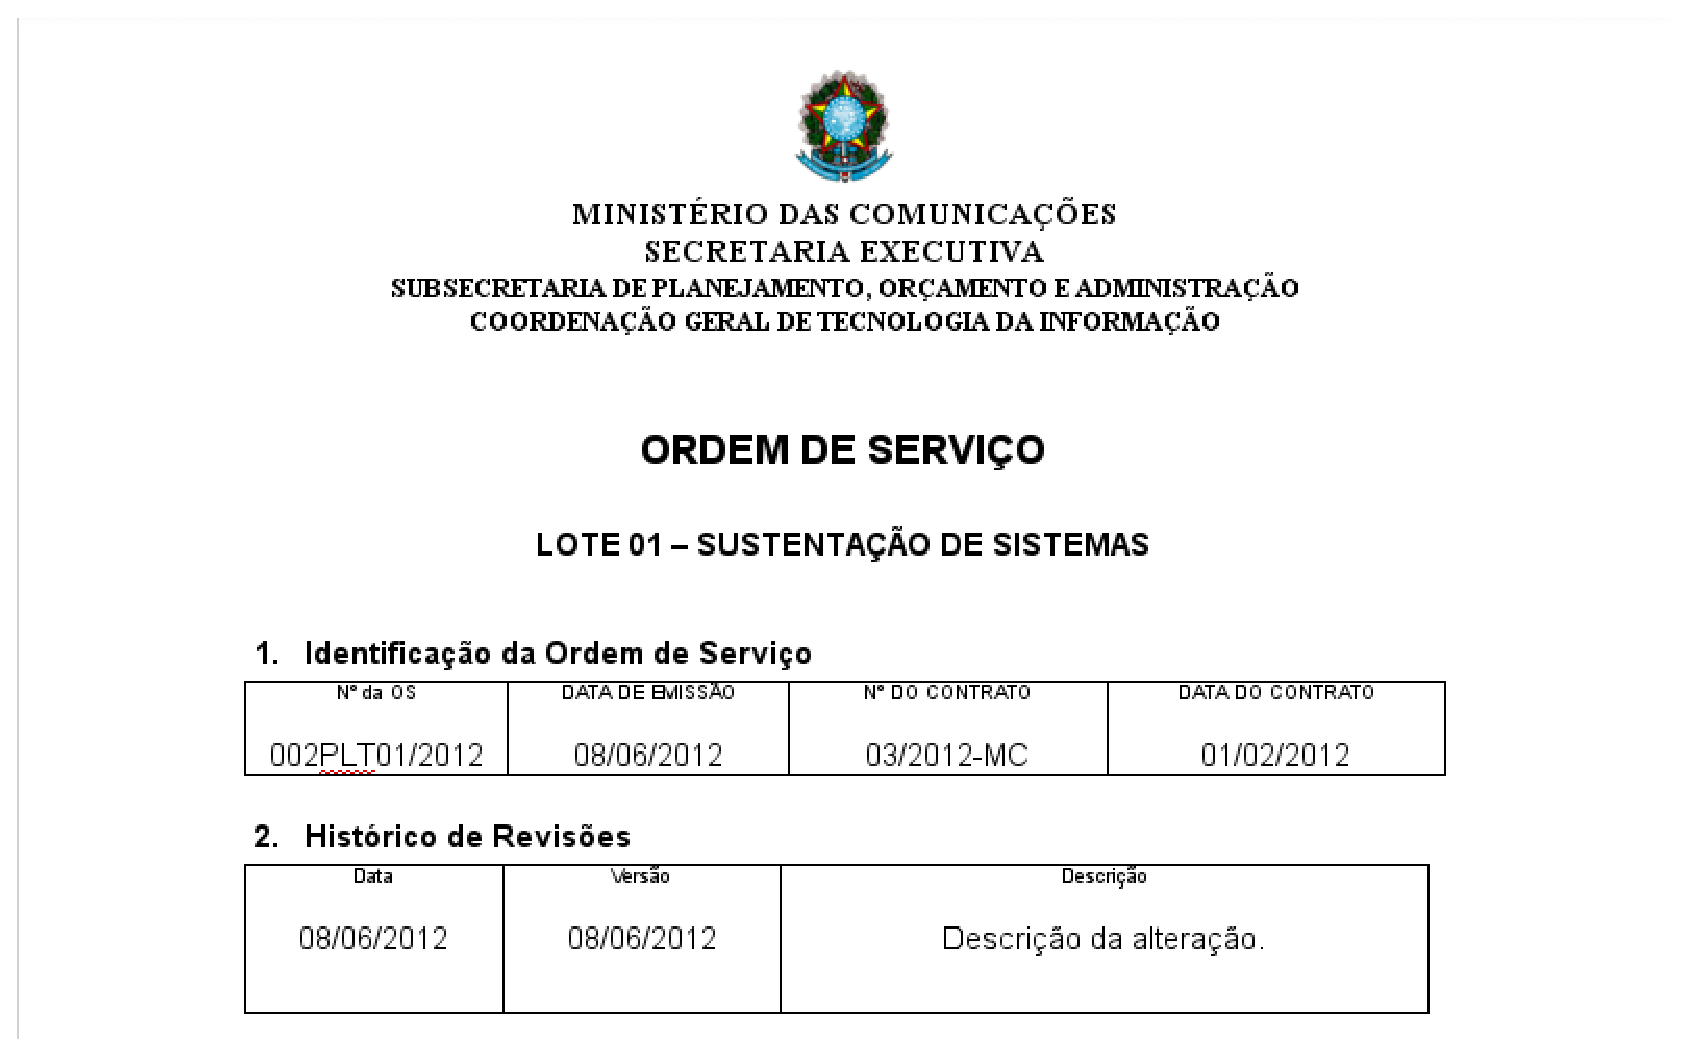
\includegraphics[keepaspectratio=true,scale=0.5]{figures/cabecalho_1_2}
  \caption{Informações básicas de uma OS \label{fig:cabecalho_1_2}}
\end{figure}

Os tópicos 3 e 4 do documento, representados pela Figura \ref{fig:pt3_4_5}, documenta
pontos relacionados à descrição das atividades associadas à OS, bem como um portfólio
dos sistemas a serem sustentados pela Fábrica contratada, uma lista de serviços a serem
realizados e a contagem total dos pontos de função envolvidos nessa ordem de serviço.

\begin{figure}[H]
  \centering
  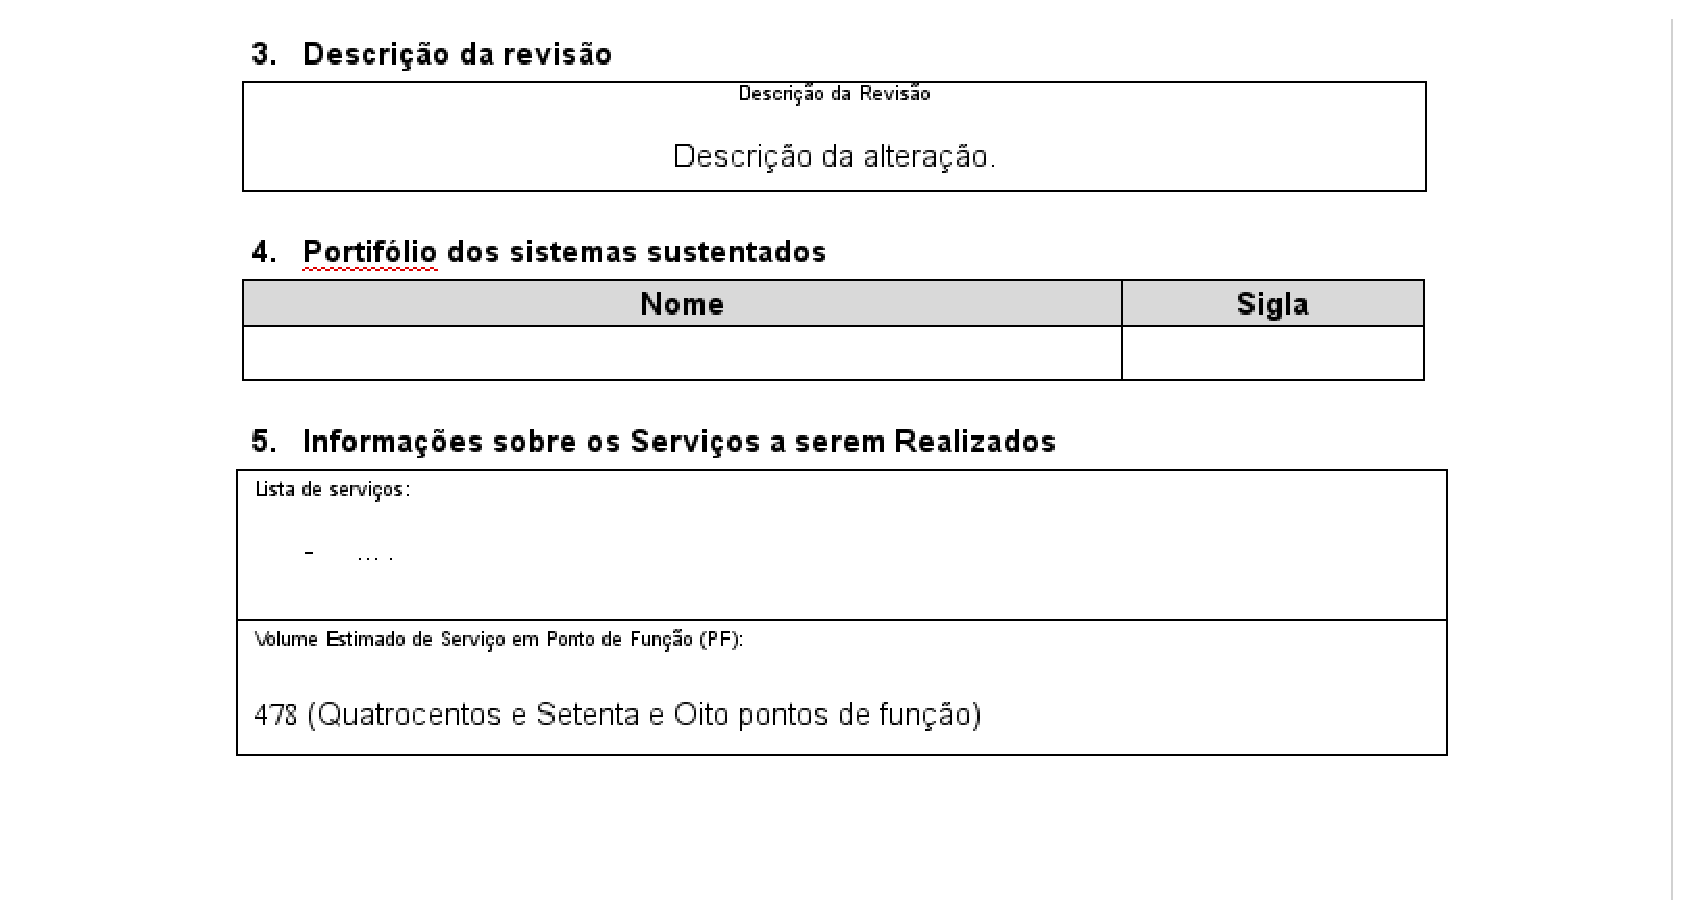
\includegraphics[keepaspectratio=true,scale=0.5]{figures/pt3_4_5}
  \caption{Descrição das atividades, portfólio e informações dos sistemas \label{fig:pt3_4_5}}
\end{figure}

Os tópicos 6 e 7, representados na Figura \ref{fig:pt6_7}, informam os custos envolvidos
e quem é o solicitante do serviço a ser executado.

\begin{figure}[H]
  \centering
  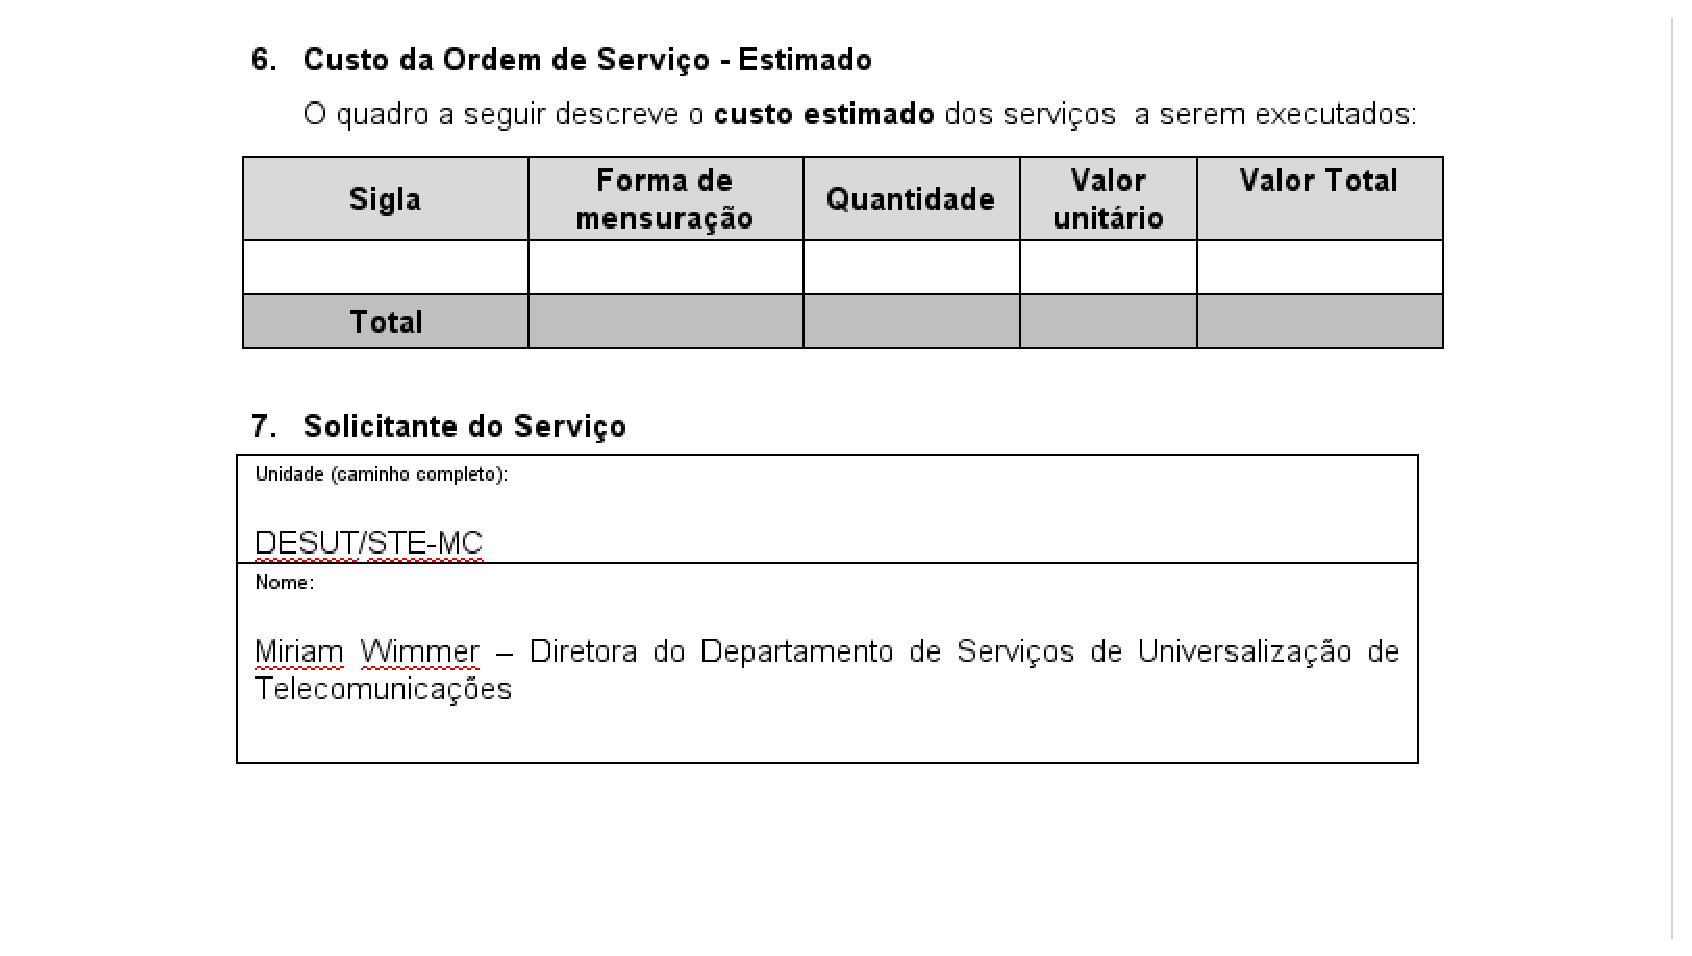
\includegraphics[keepaspectratio=true,scale=0.5]{figures/pt6_7}
  \caption{Custos e solicitante do serviço \label{fig:pt6_7}}
\end{figure}

O tópico 8, representado na Figura \ref{fig:pt8}, é designado para ter a assinatura
dos envolvidos na ordem de serviço emitida.

\begin{figure}[H]
  \centering
  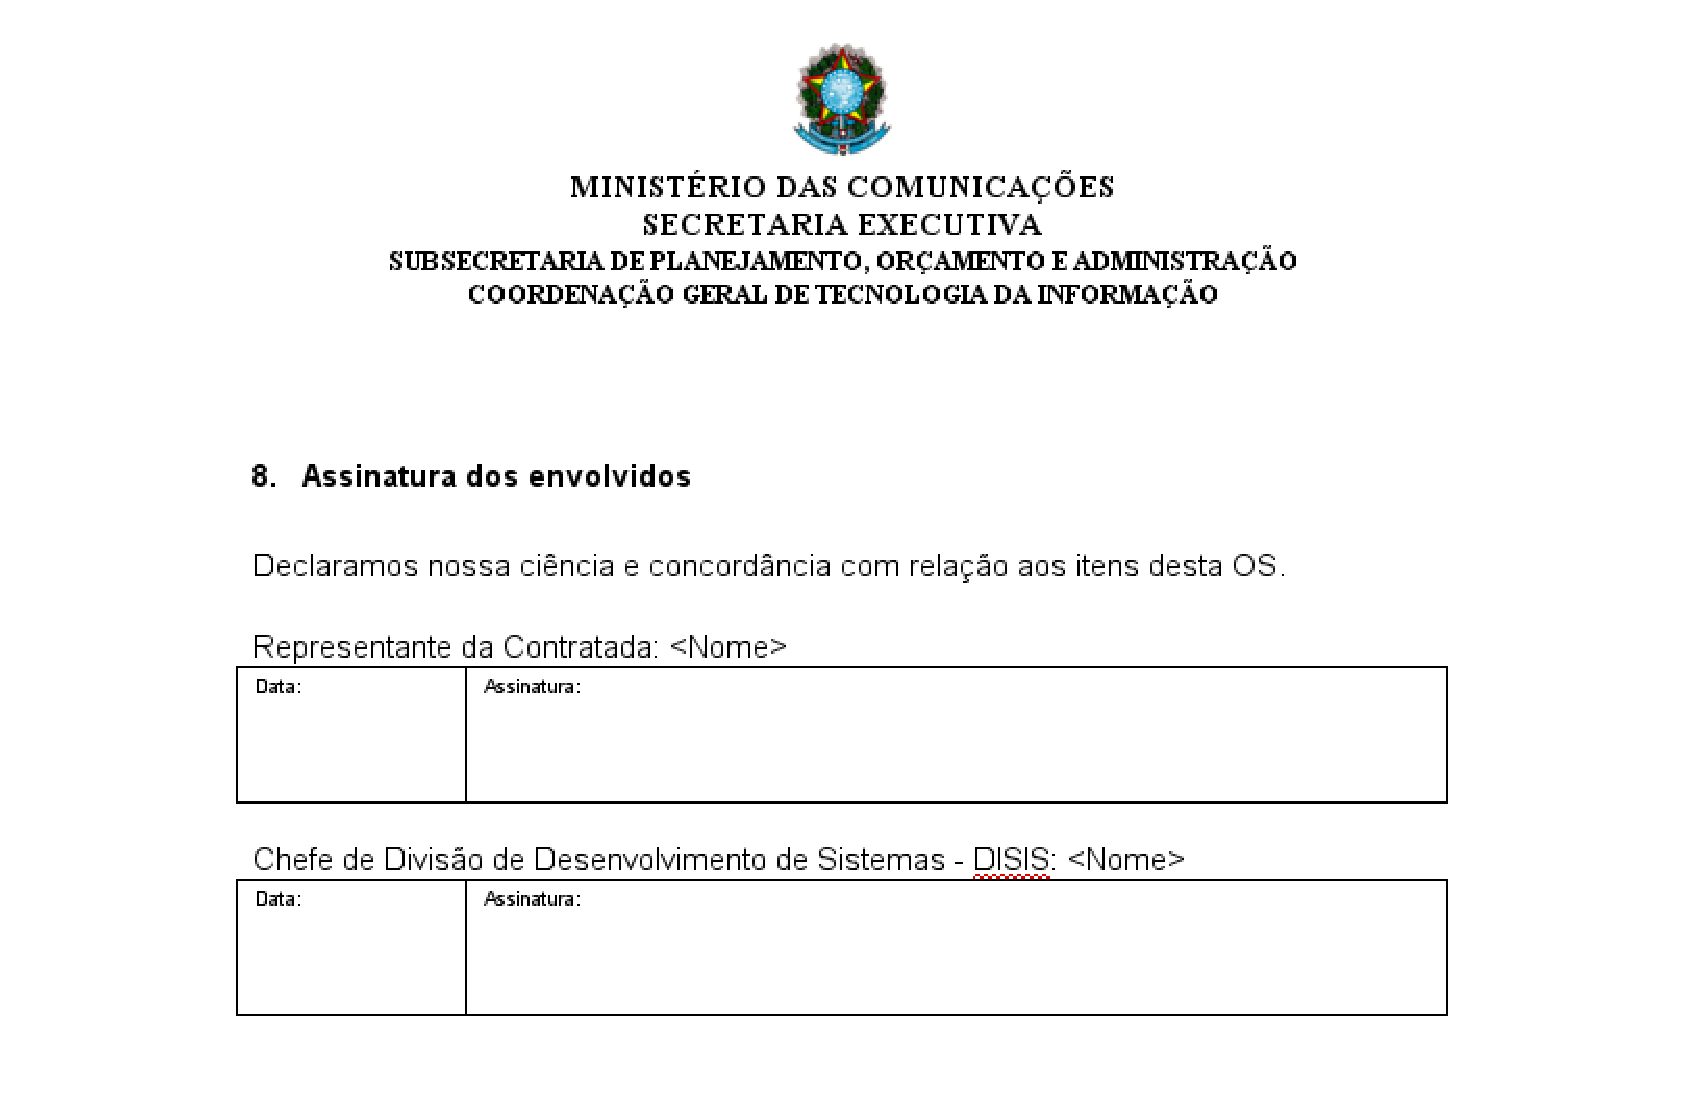
\includegraphics[keepaspectratio=true,scale=0.5]{figures/pt8}
  \caption{Assinatura dos envolvidos \label{fig:pt8}}
\end{figure}